\section[消除未知量]{消除未知量\\Elimination of Unknowns}
   \subsection{$A$ Classical Procedure}
   
\begin{flushleft}
	Now we want to describe how to eliminate an unknown from a least-squares problem. Some unknowns may be of very little importance. They are introduced into a least-squares problem in order to treat correlation in a proper way; but otherwise these unknowns are of no interest. Sometimes such unknowns are called \textit{nuisance} parameters, like the orientation unknowns in direction observations made by theodolite.
\end{flushleft}

  To begin with we will assume that all observation equations have weight 1; otherwise they would be normalized by the square root of the actual weight.

The actual procedure is easily described by means of a concrete example:
\begin{align}
\begin{bmatrix}
1    &    0\\
1    &    1\\
1    &    3\\
1    &    4
\end{bmatrix}
\begin{bmatrix}
c\\
d
\end{bmatrix}  = 
\begin{bmatrix}
0\\
8\\
8\\
20
\end{bmatrix}
- \textbf{\textit{e}}.
\end{align}
The normal equations are
\begin{align}
\begin{bmatrix}
4  &  8\\
8  &  26
\end{bmatrix}
\begin{bmatrix}
c\\
d
\end{bmatrix} = 
\begin{bmatrix}
36\\
112
\end{bmatrix}
\end{align}
and the solution is
\begin{align*}
\begin{bmatrix}
c\\
d
\end{bmatrix} =
\begin{bmatrix}
1\\
4
\end{bmatrix}.
\end{align*}
If we solve the equations according to the method of Cholesky the computations run as follows:

\begin{adjustwidth}{2em}{2em}
	Triangular decomposition of the left side
\end{adjustwidth}
\begin{align*}
l_{11} &= \sqrt{4} = 2 \\
l_{21} &=  8/2     = 4   \quad    l_{22} = \sqrt{26 - 16}  = \sqrt{10}
\end{align*}
\begin{adjustwidth}{2em}{2em}
	Forward elimination on the right side
\end{adjustwidth}
\begin{align*}
z_{1} &= 36/2 = 18 \\
z_{2} &=  (112 - 4\cdot18) /\sqrt{10}  = 40 /\sqrt{10}
\end{align*}
\begin{adjustwidth}{2em}{2em}
	Back solution 
\end{adjustwidth}
\begin{align*}
d &= 40/(\sqrt{10}\cdot\sqrt{10}) = 4 \\
c &=  (18 - 4\cdot 4) / 2  = 1.
\end{align*}
\begin{flushleft}
	Starting from this example we shall study the following trick: We augment the existing observation equations with a fictitious equation. It is the sum of the given equations and
	it is assigned the weight $ c_{fict} = -\dfrac{1}{t} = - \dfrac{1}{4}$. (The sum of the identical entries in the first 
	column of $A$ is $t$.) This new equation is
\end{flushleft}
\begin{align}
4c+8d = 36 \quad \text{with weight} \quad -\dfrac{1}{4}.
\end{align}
The augmented normal equation system has a singular matrix $A^{T}CA$:
\begin{align*}
\begin{bmatrix}
1 & 1 & 1 & 1 & 4 \\
0 & 1 & 3 & 4 & 8 
\end{bmatrix}
\begin{bmatrix}
1 &  &  &  &  \\
& 1  &  &  &  \\
& &  1  &  &  \\
& &  &  1  &  \\
& &  &  &  -\dfrac{1}{4}  
\end{bmatrix}
\begin{bmatrix}
1 & 0\\
1 & 1\\
1 & 3\\
1 & 4\\
4 & 8
\end{bmatrix} = 
\begin{bmatrix}
0 & 0\\
0 & 10
\end{bmatrix}.
\end{align*}
The system $ A^{T}CA\textbf{\textit{x}} = A^{T}C\textbf{\textit{b}}$ is still solvable (always):
\begin{align}
\begin{bmatrix}
0 & 0\\
0 & 10
\end{bmatrix}
\begin{bmatrix}
c\\
d
\end{bmatrix} = 
\begin{bmatrix}
0\\
40
\end{bmatrix}
\end{align}
which yields $d = 4$. By insertion into (6.43) we get $c$ = 1. At firat sight the singular normal equations (6.44) have a surprising structure which we want to illustrate.

Comparing the two systems of normal equations (6.42) and (6.44) it becomes evident that the unknown $c$ has been eliminated.Our earlier standard method of elimination was elementary row operations. We demonstrate the method on the actual numbers:

\begin{align}
\begin{aligned}
4c+8d & = & 36 \\
8c+26d & = & 112
\end{aligned}  \quad 
\rightarrow    \quad 
\begin{aligned}
4c+8d & = & 36\\
10d   & = & 40,
\end{aligned}
\end{align}
and this reveals nothing view.

Earlier we assumed that all entries are identical in the column of $A$ corresponding to the unknown to be eliminated. In practice these entries often are 1.

If the weights $c_{i}$ of the single obsernations are varying then the weight of the fictitious equation has to be changed to $ c_{fict} = -1/\Sigma^{m}_{i=1}c_{i}$ and the summation in $A$ has to be performed as a weighted summation. 

The variance $ \sigma^{2}_{c}$ of the eliminated unknown $c$ is calculated as follows: In order to calculate the inverse matrix of the norm equations we use the same row operations as above on the unit matrix:
\begin{align*}
\begin{bmatrix}
1 & 0\\
0 & 1
\end{bmatrix}
\quad
\rightarrow
\quad
\begin{bmatrix}
1 & 0\\
-2 & 1
\end{bmatrix}.
\end{align*}
We substitute the first column as right side in (6.45) and obtain the solution
\begin{align*}
\textbf{\textit{v}}_{1} = 
\begin{bmatrix}
\dfrac{13}{20}\\
-\dfrac{1}{5}
\end{bmatrix}
\end{align*}
and substituting the second column as right side yields the following solution
\begin{align*}
\textbf{\textit{v}}_{2} = 
\begin{bmatrix}
-\dfrac{1}{5}\\
\dfrac{1}{10}
\end{bmatrix}
\end{align*}
or
\begin{align*}
(A^{T}CA)^{-1} = 
\begin{bmatrix}
\textbf{\textit{v}}_{1} & \textbf{\textit{v}}_{2}
 \end{bmatrix} =
 \dfrac{1}{20}
 \begin{bmatrix}
13 & -4\\
-4 & 2 
 \end{bmatrix}.
\end{align*}
This result, of course, is also obtained when using ordinary methods for the inversion of the coefficient matrix (6.42).

In order to calculate the variance factor $  \hat{\alpha}^{2}_{0} $ we have to use (4.86)
\begin{align*}
\hat{\textbf{\textit{e}}}^{T}C \hat{\textbf{\textit{e}}} =
\textbf{\textit{b}}^{T}C\textbf{\textit{b}} - \textbf{\textit{z}}^{T}\textbf{\textit{z}} = \textbf{\textit{b}}^{T}C\textbf{\textit{b}} -
\Sigma z^{2}_{i} = 64 + 64 + 400 - (324 + 160) = 44.
\end{align*}
An identical result is produced by calculating
\begin{align*}
\textbf{\textit{p}} = A\hat{\textbf{\textit{x}}} =
\begin{bmatrix}
1\\
5\\
13\\
17
\end{bmatrix} \quad
and then \quad
\hat{\textbf{\textit{e}}} = \textbf{\textit{b}} - \textbf{\textit{p}} =
\begin{bmatrix}
-1\\
3\\
-5\\
3
\end{bmatrix}.
\end{align*}
Subsequently, $ \hat{\sigma}^{2}_{0} = 44/(4-2) = 22$. Note that $n$ is not to be reduced because of the elimination. Implicitly there still are $n$ unknown. Finally
\begin{align*}
\hat{\sigma}^{2}_{c} = \dfrac{22\cdot 26}{40} = 14.3 
\quad 
and
\quad
\hat{\sigma}^{2}_{d} = \dfrac{22\cdot 4}{40} = 2.2. 
\end{align*}
We summarize the method: In a least-squares problem we want to eliminate an unknown with constant coefficients. This is done by augmenting the original problem with a fictitious observation equation which results as the sum of all observation equations in which this unknown appears. The new equation is given the weight -1/(sum of coefficients of the unknown). Next, the remaining $n-1$ normal equations are solved in usual manner. Subsequently, the eliminated unknown can be calculated from the new observation equation by insertion of the solution. The variance of the unknown is calculated from the normal equations by using unit vectors as right sides and by using the same row operations as for the elimination of the unknown.

\subsection{Eliminating From the Normal Equations}
\begin{flushleft}
	We want to make the above description more general and cogent by using the technique of \textit{block elimination}. Let the normal equations be split as follows (remember $B=C^{T}$):
\end{flushleft}
\begin{align*}
\begin{bmatrix}
A  & B\\
C  & D
\end{bmatrix}
\begin{bmatrix}
\textbf{\textit{x}}_{1}\\
\textbf{\textit{x}}_{2}
\end{bmatrix} =
\begin{bmatrix}
\textbf{\textit{b}}_{1}\\
\textbf{\textit{b}}_{2}
\end{bmatrix}.
\end{align*}
Block elimination subtracts $CA^{-1}$ times the first row $[A B]$ and $\textbf{\textit{b}}_{1}$. This is achieved by multiplying to the left with the elimination matrix:
\begin{align*}
\begin{bmatrix}
I  &  0\\
-CA^{-1} & I
\end{bmatrix}
\begin{bmatrix}
A  &  B\\
C &   D
\end{bmatrix}
\begin{bmatrix}
\textbf{\textit{x}}_{1}\\
\textbf{\textit{x}}_{2}
\end{bmatrix} =
\begin{bmatrix}
I  &  0\\
-CA^{-1} & I
\end{bmatrix}
\begin{bmatrix}
\textbf{\textit{b}}_{1}\\
\textbf{\textit{b}}_{2}
\end{bmatrix}
\end{align*}
or explicitly
\begin{align*}
\begin{bmatrix}
A & B\\
0 & D-CA^{-1}B
\end{bmatrix}
\begin{bmatrix}
\textbf{\textit{x}}_{1}\\
\textbf{\textit{x}}_{2}
\end{bmatrix}
=
\begin{bmatrix}
\textbf{\textit{b}}_{1}\\
\textbf{\textit{b}}_{2} - CA^{-1}\textbf{\textit{b}}_{1}
\end{bmatrix}.
\end{align*}
The last row contains the wanted expression for the remaining unknown:
\begin{align}
\textbf{\textit{x}}_{2} = (D-CA^{-1}B)^{-1}(\textbf{\textit{b}}_{2} - CA^{-1}\textbf{\textit{b}}_{1}).
\end{align}
This formula is coded as the $M$-file elimnor.

\subsection{Eliminating Parameters: $A$ Reduced Estimation Problem}

\begin{flushleft}
	Suppose the vector $\textbf{\textit{x}}$ of modeling parameters is separated into an unimportant part $\textbf{\textit{y}}$ and an important part $z$. Then we can eliminate $\hat{\textbf{\textit{y}}}$ from the normal equations and solve only for $\hat{z}$. And we can return to find $\hat{\textbf{\textit{y}}}$ if we want. It is useful to describe those steps.
\end{flushleft}

We will execute a standard elimination of $\hat{\textbf{\textit{y}}}$ from the normal equations for $\hat{\textbf{\textit{x}}} = [\hat{\textbf{\textit{y}}} \ \hat{\textbf{\textit{z}}}]$. Start with the observation equations
\begin{align}
\textbf{\textit{b}} = A\textbf{\textit{x}} + \textbf{\textit{e}} = B \textbf{\textit{y}} + Gz + \textbf{\textit{e}}.
\end{align}
Denote the weight matrix $ \Sigma ^{-1}_{b}$ by $C$. The normal equations are
\begin{align}
\begin{bmatrix}
B^{T}\\
G^{T}
\end{bmatrix} C
\begin{bmatrix}
B & G
\end{bmatrix}
\begin{bmatrix}
\hat{\textbf{\textit{y}}}\\
\hat{\textbf{\textit{z}}}
\end{bmatrix} = 
\begin{bmatrix}
B^{T}\\
G^{T}
\end{bmatrix} C \textbf{\textit{b}}.
\end{align}
This produces two block equations for $\hat{\textbf{\textit{y}}}$ and $\hat{\textbf{\textit{z}}}$:
\begin{align}
\begin{bmatrix}
B^{T}CB & B^{T}CG \\
G^{T}CB & G^{T}CG
\end{bmatrix}
\begin{bmatrix}
\hat{\textbf{\textit{y}}}\\
\hat{\textbf{\textit{z}}}
\end{bmatrix} =
\begin{bmatrix}
B^{T}C \textbf{\textit{b}}\\
G^{T}C \textbf{\textit{b}}
\end{bmatrix}.
\end{align}
To eliminate $\hat{\textbf{\textit{y}}}$, multiply row 1 by $G^{T}CB(B^{T}CB)^{-1}$ and subtract from row 2. This produces a zero block in row 2, column 1 .It leaves an equation for $\hat{\textbf{\textit{z}}}$ alone, with a \textit{modified weighting matrix} $C'$:
\begin{align}
G^{T}C'G\hat{z} = G^{T}C'\textbf{\textit{b}} \quad
with
\quad
C' = C - CB(B^{T}CB)^{-1}B^{T}C.
\end{align}
Note that $C'B$ is the zero matrix. The algebra has confirmed what we could have expected: the reduced model for $\hat{z}$ alone has a smaller weight matrix $C'$ (and a larger covariance matrix) because the $B \ \textbf{\textit{y}}$ term is projected out. As always, back substitution in (6.49) yields $\hat{\textbf{\textit{y}}}$ when we know $\hat{\textbf{\textit{z}}}$:
\begin{align}
\hat{\textbf{\textit{y}}} = (B^{T}CB)^{-1}B^{T}C(\textbf{\textit{b}} - G\hat{z} )
\end{align}
\begin{figure}[htb]
	\centering
	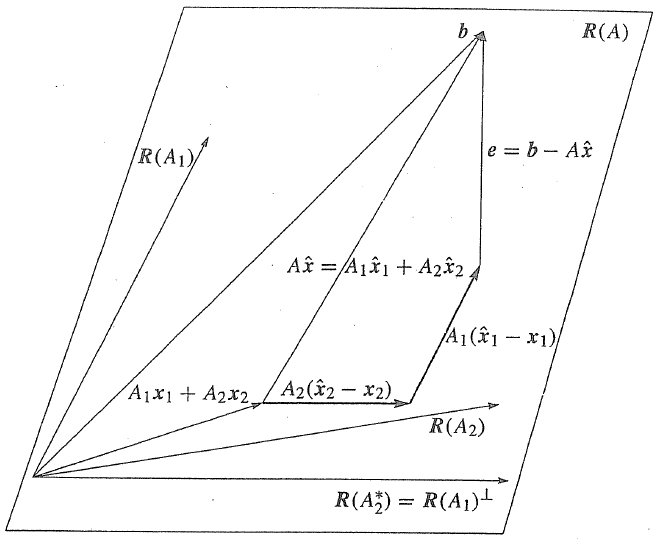
\includegraphics[width=0.7\linewidth]{TeX_files/Part02/chapter06/image/6-3}
	\caption{Geometry of the orthogonal decomposition in the column space $\textbf{R}(A)$ of $A=[A1 \ A2]$ }
\end{figure}


\subsection{Eliminating From the Observation Equations}

\begin{flushleft}
	If we use the above procedure directly on the observation equations it works formally, but we generally get a wrong result. The column space must be split into two subspaces conforming to the splitting of $A$ into$[A1 \ A2]$,and furthermore, the two subspaces must be orthogonal complements.
\end{flushleft}

First, partition the observation equations into
\begin{align}
\begin{bmatrix}
A_{1}\\
A_{2}
\end{bmatrix}
\begin{bmatrix}
\textbf{\textit{x}}_{1} & \textbf{\textit{x}}_{2}
\end{bmatrix} = \textbf{\textit{b}}.
\end{align}
The columns of $A = [A1 \ A2]$ span $\textbf{R}(A)$. We decompose $\textbf{R}(A)$ into the space $\textbf{R}(A_{1})$ spanned by the columns of $A_{1}$ and its orthogonal complement $\textbf{R}^{\bot} $. By definition we have $ A^{T}_{1}CA^{*}_{2} = 0 $ where $ A^{*}_{2}$ spans $\textbf{R}^{\bot} $.

The projector $P = I -A_{1}(A^{T}_{1}CA_{1})^{-1}A^{T}_{1}C $ projects $A_{2}$ in $\textbf{R}(A)$ to $ A^{*}_{2}$ in $\textbf{R}^{\bot} $:
\begin{align*}
A^{*}_{2} = (I -A_{1}(A^{T}_{1}CA_{1})^{-1}A^{T}_{1}C)A_{2}.
\end{align*}
The reduced observation equations are
\begin{align*}
(I -A_{1}(A^{T}_{1}CA_{1})^{-1}A^{T}_{1}C)A_{2}\textbf{\textit{x}}_{2} =
(I -A_{1}(A^{T}_{1}CA_{1})^{-1}A^{T}_{1}C)\textbf{\textit{b}}
\end{align*}
or abbreviated
\begin{align*}
A^{*}_{2}\textbf{\textit{x}}_{2} = \textbf{\textit{b}}^{*}.
\end{align*}
Next we solve for $ \textbf{\textit{x}}_{2}$:
\begin{align}
\textbf{\textit{x}}_{2} = ( A^{*^T}_{2}CA^{*}_{2} )^{-1}A^{*^T}_{2}C \textbf{\textit{b}}^{*}.
\end{align}
The above procedure has important applications. When processing $GPS$ observations may want to eliminate the ambiguity unknowns. We rewrite (6.52) as
\begin{align*}
A_{1}\textbf{\textit{x}}_{1} + A_{2}\textbf{\textit{x}}_{2} = \textbf{\textit{b}}.
\end{align*}
The unknowns $ \textbf{\textit{x}}_{1}$ are eliminated by multiplication by the projector $\textbf{P}$ onto $ \textbf{R}^{\bot}$:
\begin{align*}
PA_{1}\textbf{\textit{x}}_{1} + PA_{2}\textbf{\textit{x}}_{2} = P\textbf{\textit{b}}.
\end{align*}
As $PA_{1}=0$ the transformed observation equations become
\begin{align*}
A^{*}_{2}\textbf{\textit{x}}_{2}= \textbf{\textit{b}}^{*}.
\end{align*}
We depict the geometry of this orthogonal decomposition in Figure 6.3.

Finally we want to demonstrate the procedure on the observations from (6.41). The coefficient matrix $A$ is split into the two columns $[A1 A2]$.Hence the projector $P$ becomes
\begin{align*}
P = \dfrac{1}{4}
\begin{bmatrix}
3 & -1 & -1 & -1 \\
-1 & 3 & -1 & -1 \\
-1 & -1 & 3 & -1 \\
-1 & -1 & -1 & 3 
\end{bmatrix}.
\end{align*}
The transformed observation equations $A^{*}_{2}\textbf{\textit{x}}_{2} = \textbf{\textit{b}}^{*} $ are
\begin{align*}
\begin{bmatrix}
-2 \\
 -1 \\
1 \\
2 
\end{bmatrix}
\textbf{\textit{x}}_{2}= 
\begin{bmatrix}
-9 \\
-1 \\
-1 \\
11 
\end{bmatrix}.
\end{align*}
The normals are $ 10\hat{\textbf{\textit{x}}}_{2} = 40$ and the solution is again recovered as $\hat{\textbf{\textit{x}}}_{2} = 4 $.

The error calculation runs as follows:

\begin{align*}
\hat{\textbf{\textit{e}}} = \textbf{\textit{b}}^{*} -A^{*}_{2} \hat{\textbf{\textit{x}}}_{2} =
\begin{bmatrix}
-9 \\
-1 \\
-1 \\
11 
\end{bmatrix} -
\begin{bmatrix}
-2 \\
-1 \\
1 \\
2 
\end{bmatrix}4 = 
\begin{bmatrix}
-1 \\
3 \\
-5 \\
3 
\end{bmatrix};
\end{align*}
And
\begin{align*}
\hat{\sigma}^{2}_{0} = \dfrac{44}{4-2} = 22 .
\end{align*}
The procedure is coded in the $M$-file elimobs.